% SPDX-FileCopyrightText: 2026 Onur Tuncer and Stereon contributors
% SPDX-License-Identifier: MPL-2.0
%
% This Source Code Form is subject to the terms of the Mozilla Public
% License, v. 2.0. If a copy of the MPL was not distributed with this
% file, You can obtain one at https://mozilla.org/MPL/2.0/.
%
% ADR-0001's containment invariant (docs/tolerances.rst): an edge's
% tolerance tube of radius tau_e about its reference trace holds every
% other trace of the edge, each pcurve mapped through its surface (rule
% G02); each vertex's tolerance sphere of radius tau_v holds the ends of
% the edges that meet there (rule G01).
\documentclass[tikz,border=6pt]{standalone}
\usepackage{amsmath}
\usetikzlibrary{calc,arrows.meta,decorations.pathreplacing}
\definecolor{ref}{RGB}{31,119,180}
\definecolor{trace}{RGB}{214,39,40}
\definecolor{tube}{RGB}{31,119,180}
\definecolor{vert}{RGB}{44,160,44}
\begin{document}
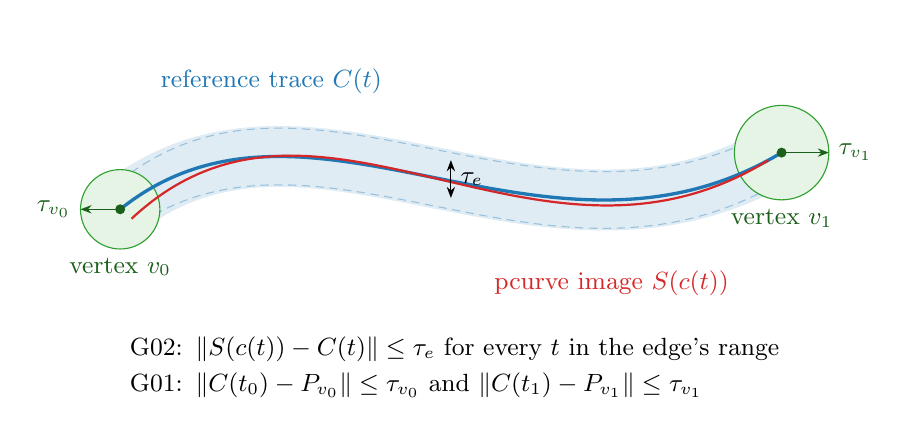
\begin{tikzpicture}[scale=1.2,lbl/.style={font=\small}]
  % The reference trace: C(t), or S_1(c_1(t)) for an edge without a curve
  \def\refpath{(0,0) .. controls (2,1.6) and (4.5,-0.9) .. (7,0.6)}
  % The tube: the reference path stroked wide, drawn first
  \draw[line width=22pt,tube!14,line cap=round] \refpath;
  \draw[tube!45,densely dashed] (0,0.3) .. controls (2,1.9) and (4.5,-0.6) .. (7,0.9);
  \draw[tube!45,densely dashed] (0,-0.3) .. controls (2,1.3) and (4.5,-1.2) .. (7,0.3);
  % The vertex spheres
  \draw[vert,fill=vert!12] (0,0) circle (0.42);
  \draw[vert,fill=vert!12] (7,0.6) circle (0.5);
  % The reference trace and a second trace, inside the tube
  \draw[ref,very thick] \refpath;
  \draw[trace,thick] (0.12,-0.1) .. controls (2.1,1.75) and (4.4,-1.0) .. (6.86,0.52);
  % The vertices
  \fill[vert!60!black] (0,0) circle (1.5pt);
  \fill[vert!60!black] (7,0.6) circle (1.5pt);
  % Radii
  \draw[{Stealth[length=4pt]}-{Stealth[length=4pt]}] (3.5,0.12) -- (3.5,0.52)
      node[lbl,right,midway] {$\tau_e$};
  \draw[vert!60!black,-{Stealth[length=4pt]}] (7,0.6) -- (7.5,0.6) node[lbl,right] {$\tau_{v_1}$};
  \draw[vert!60!black,-{Stealth[length=4pt]}] (0,0) -- (-0.42,0) node[lbl,left] {$\tau_{v_0}$};
  % Labels
  \node[lbl,ref,above] at (1.6,1.12) {reference trace $C(t)$};
  \node[lbl,trace,below] at (5.2,-0.55) {pcurve image $S(c(t))$};
  \node[lbl,vert!60!black,below=14pt] at (0,0) {vertex $v_0$};
  \node[lbl,vert!60!black,below=17pt] at (7,0.6) {vertex $v_1$};
  % The conditions
  \node[lbl,align=left,anchor=north west] at (0,-1.25) {%
    G02:\enspace $\lVert S(c(t)) - C(t)\rVert \le \tau_e$ for every $t$ in the edge's range\\[2pt]
    G01:\enspace $\lVert C(t_0) - P_{v_0}\rVert \le \tau_{v_0}$ and
    $\lVert C(t_1) - P_{v_1}\rVert \le \tau_{v_1}$};
\end{tikzpicture}
\end{document}
